The lenet model was implemented in the keras which requires the input image of 32 * 32 pixels. As, a result 
all the pre processing and normalisation was performed on images of pigmented skin lesion on required sizes.
The lenet architecture was easy to train and required less time to learn the relationship in the given data becuase 
of the light network architecture and images of low dimensions.

\begin{figure}[!htp]
    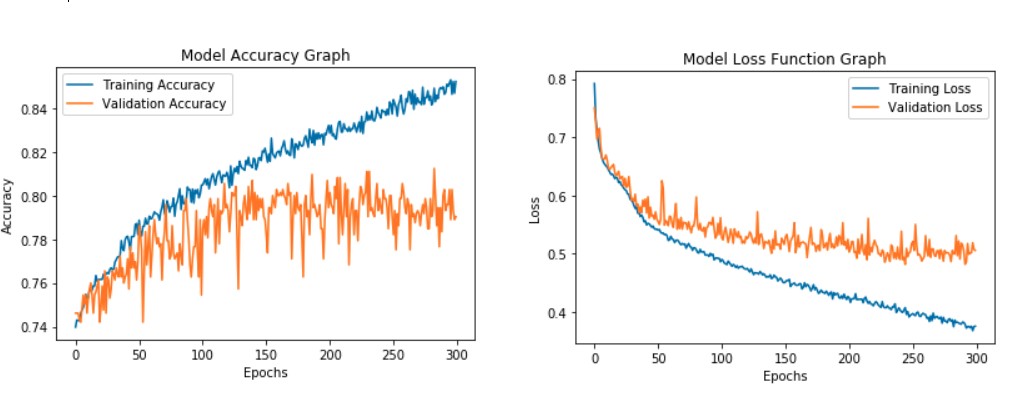
\includegraphics[width=\textwidth]{Images/lenetarc.png}
    \caption{Lenet Model training}
    \label{fig:llenet}
\end{figure}

The figure \ref{fig:llenet} shows the model accuracy and loss function graph of the first experiment 
performed on the lenet model architecture with SGD optimiser and learning rate of 0.01 for 300 epochs. 
The result obtained from accuracy of the evaluation performed on the testing data was 80.35\%.
However, the traditional method of training the lenet model architecture requires using 
Adam optimiser with learning rate of 0.0001 and resulted in better accuracy evaluation of 81.34\% on testing data.

\begin{figure}[!htp]
    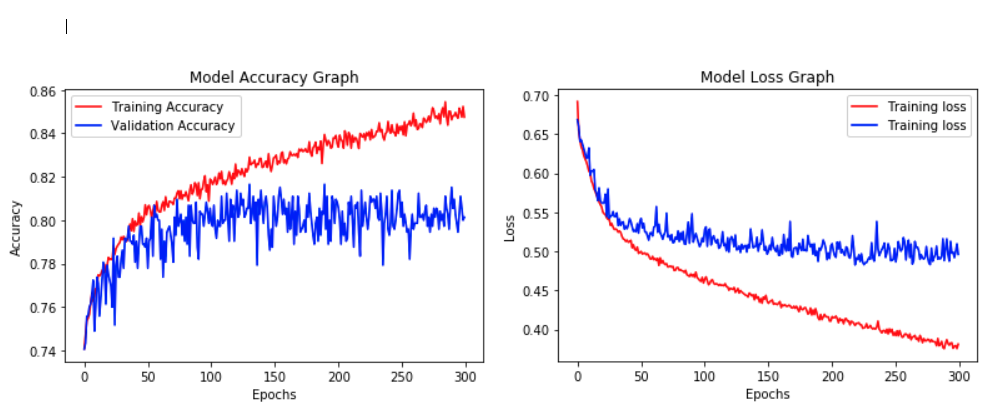
\includegraphics[width=\textwidth]{Images/lenet22.png}
    \caption{Transfer Learning Lenet Model training}
    \label{fig:lenet22}
\end{figure}

The figure \ref{fig:lenet22} show the model training training performed using the transfer learning on the 
lenet in attempt to achieve better model accuracy results. The model accuracy obtained from the transfer learning approch on 
lenet architecture was 81.56\% on testing data. Therefore, it was most sucessful model so, far in analysing the 
categories of pigmented skin lesions. However, the lenet architecture only functions on small image size of 
32 * 32 pixels which when resized might loose vitial information in the process of diagnosing pigmented skin lesions.